%==============================================================================
% Chapitre 30 - Stabilité statique
%==============================================================================

\section{Introduction}

Au cours de son vol, un projectile n'est jamais parfaitement aligné avec sa
trajectoire.

De petites perturbations apparaissent constamment :

\begin{itemize}
    \item rafales de vent ;
    \item turbulences ;
    \item imperfections géométriques ;
    \item vibrations ;
    \item perturbations de sortie de bouche.
\end{itemize}

La stabilité statique décrit la manière dont le projectile réagit à ces
perturbations initiales.

\begin{aretenir}

La stabilité statique indique si une perturbation tend à diminuer ou à
s'amplifier.

\end{aretenir}

\section{Position d'équilibre}

Considérons un projectile parfaitement aligné avec sa trajectoire.

Dans cette situation :

\begin{itemize}
    \item l'incidence est nulle ;
    \item les forces latérales sont minimales ;
    \item les moments aérodynamiques sont faibles.
\end{itemize}

Cette configuration constitue la position d'équilibre.

\section{Perturbation}

Supposons maintenant qu'une petite perturbation apparaisse.

Le projectile prend alors une faible incidence par rapport à son écoulement.

L'air exerce immédiatement de nouvelles forces aérodynamiques.

La question fondamentale devient :

\begin{quote}
Ces forces vont-elles corriger la perturbation ou l'amplifier ?
\end{quote}

\section{Définition de la stabilité statique}

Un système est dit statiquement stable si une perturbation provoque une
réaction tendant à ramener le système vers son état d'équilibre.

À l'inverse, il est statiquement instable si la perturbation tend à
s'amplifier.

\section{Exemple : une bille dans une cuvette}

Une analogie classique consiste à considérer une bille placée dans une
cuvette.

Si la bille est déplacée légèrement :

\begin{itemize}
    \item elle revient naturellement vers le fond ;
    \item l'équilibre est stable.
\end{itemize}

\section{Exemple : une bille sur une colline}

Considérons maintenant une bille placée au sommet d'une colline.

Une petite perturbation provoque :

\begin{itemize}
    \item son éloignement du point initial ;
    \item une amplification du mouvement.
\end{itemize}

L'équilibre est alors instable.

\section{Application aux projectiles}

Pour un projectile, la stabilité dépend principalement de la position
relative :

\begin{itemize}
    \item du centre de gravité ;
    \item du centre de pression.
\end{itemize}

Ces deux points déterminent le signe du moment aérodynamique produit par une
perturbation.

\section{Moment restaurateur}

Lorsqu'une perturbation génère un moment qui tend à réaligner le projectile,
on parle de moment restaurateur.

Le projectile tend alors à revenir vers sa position d'équilibre.

Cette situation correspond à une stabilité statique.

\begin{figure}[htbp]
\centering
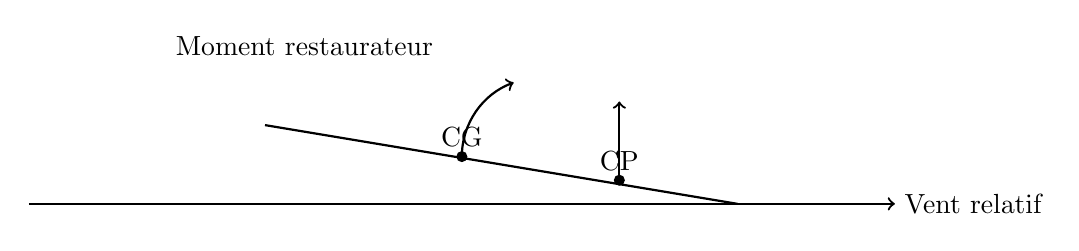
\begin{tikzpicture}

\draw[thick,->] (-1,0) -- (10,0);
\node[right] at (10,0) {Vent relatif};

\draw[thick] (2,1) -- (8,0);

\fill (4.5,0.6) circle (2pt);
\fill (6.5,0.3) circle (2pt);

\node[above] at (4.5,0.6) {CG};
\node[above] at (6.5,0.3) {CP};

\draw[->,thick] (6.5,0.3) -- (6.5,1.3);

\draw[->,thick] (4.5,0.6) arc (180:110:1);

\node at (2.5,2) {Moment restaurateur};

\end{tikzpicture}
\caption{Principe d'un moment restaurateur.}
\label{fig:moment_restaurateur}
\end{figure}

\section{Moment déstabilisateur}

À l'inverse, si la perturbation génère un moment qui augmente encore
l'incidence :

\begin{itemize}
    \item l'écart grandit ;
    \item l'instabilité augmente.
\end{itemize}

On parle alors de moment déstabilisateur.

\section{Projectile empenné}

Les flèches constituent un excellent exemple.

Leurs empennages déplacent fortement le centre de pression vers l'arrière.

Lorsque la flèche est perturbée :

\begin{itemize}
    \item les forces aérodynamiques tendent à la réaligner ;
    \item elle retrouve naturellement son orientation.
\end{itemize}

Cette configuration présente une forte stabilité statique.

\begin{aretenir}

Les flèches sont principalement stabilisées par leur géométrie.

\end{aretenir}

\section{Projectile cylindro-ogival}

Les projectiles modernes d'armes à feu présentent une situation différente.

Leur géométrie offre :

\begin{itemize}
    \item une faible traînée ;
    \item une excellente conservation de vitesse ;
    \item mais une stabilité naturelle limitée.
\end{itemize}

La stabilisation doit alors être assurée par la rotation.

\section{Stabilité statique et stabilité dynamique}

La stabilité statique ne doit pas être confondue avec la stabilité dynamique.

La stabilité statique répond à la question :

\begin{quote}
Quelle est la réaction immédiate à une perturbation ?
\end{quote}

La stabilité dynamique étudie ensuite l'évolution du mouvement dans le temps.

\section{Importance de l'incidence}

Même une incidence très faible peut générer :

\begin{itemize}
    \item des forces aérodynamiques ;
    \item des moments importants ;
    \item des oscillations.
\end{itemize}

La stabilité dépend donc fortement de la réponse du projectile à ces faibles
angles.

\section{Marge statique}

La différence de position entre :

\begin{itemize}
    \item le centre de gravité ;
    \item le centre de pression ;
\end{itemize}

est souvent utilisée pour caractériser la stabilité.

On parle parfois de marge statique.

Plus cette marge est importante, plus la stabilité naturelle tend à être
élevée.

\section{Limites de la stabilité statique}

Une stabilité statique élevée n'est pas toujours souhaitable.

Un projectile excessivement stable peut présenter :

\begin{itemize}
    \item une traînée accrue ;
    \item une géométrie moins performante ;
    \item d'autres compromis aérodynamiques.
\end{itemize}

La conception résulte toujours d'un compromis.

\section{Conséquences pour les projectiles modernes}

Les projectiles modernes privilégient souvent :

\begin{itemize}
    \item l'aérodynamique ;
    \item la conservation de vitesse ;
    \item la portée.
\end{itemize}

La stabilité est alors obtenue principalement grâce à la rotation imposée
par les rayures.

\section{Stabilité et simulation}

Les modèles avancés prennent en compte :

\begin{itemize}
    \item les centres caractéristiques ;
    \item les moments aérodynamiques ;
    \item les coefficients de stabilité.
\end{itemize}

Ces paramètres permettent de reproduire correctement le comportement du
projectile après une perturbation.

\begin{simulation}

Les modèles de masse ponctuelle ne représentent généralement pas la stabilité
statique.

Les modèles 6DOF la calculent explicitement.

\end{simulation}

\section{Vers la stabilisation gyroscopique}

Nous savons désormais pourquoi certains projectiles sont naturellement
stables tandis que d'autres ne le sont pas.

Une question demeure :

\begin{quote}
Comment une balle moderne peut-elle rester stable alors que sa géométrie ne
l'est pas naturellement ?
\end{quote}

La réponse réside dans la rotation rapide imposée par les rayures du canon.

\section{À retenir}

\begin{aretenir}

\begin{itemize}
    \item La stabilité statique décrit la réaction initiale à une
          perturbation.
    \item Un moment restaurateur produit un comportement stable.
    \item Un moment déstabilisateur produit un comportement instable.
    \item La position relative du CG et du CP joue un rôle essentiel.
    \item Les projectiles modernes utilisent principalement la stabilisation
          gyroscopique.
\end{itemize}

\end{aretenir}
